\chapter{Introducción}

% \defaultFontEpigraph{All You Need Is a Good Init}{\cite{mishkinAllYouNeed2016}}
\defaultFontEpigraph{All You Need Is a Good Init}{Mishkin y Matas (2016)}

\todo[]{Realizar la introducción del trabajo siguiendo estos puntos.}
A realizar:
\begin{itemize}
    \item Presentar el trabajo de forma atractiva
    \begin{itemize}
        \item Traer algunas ideas de Justificación
        \item Explicar título "All You Need" y epígrafes. Nos apoyamos en la Figura \ref{fig:all_you_need_publicaciones}
        \item Este trabajo es investigación, pero tiene como fruto un software de \textit{live coding}, \textit{AI Muse} y una obra de arte sonoro, \textit{AlgoraI}
    \end{itemize}
    \item Describir los deferentes capítulos
    \item Explicar el uso de acrónimos
    \item Explicar el uso de los QR
\end{itemize}




\begin{figure}[H]
    \caption[Número de publicaciones de \textit{Deep Learning} por año que contienen la expresión <<all you need>> en el título]{Número de publicaciones de \textit{Deep Learning} por año que contienen la expresión <<all you need>> en el título.}
    \centering
    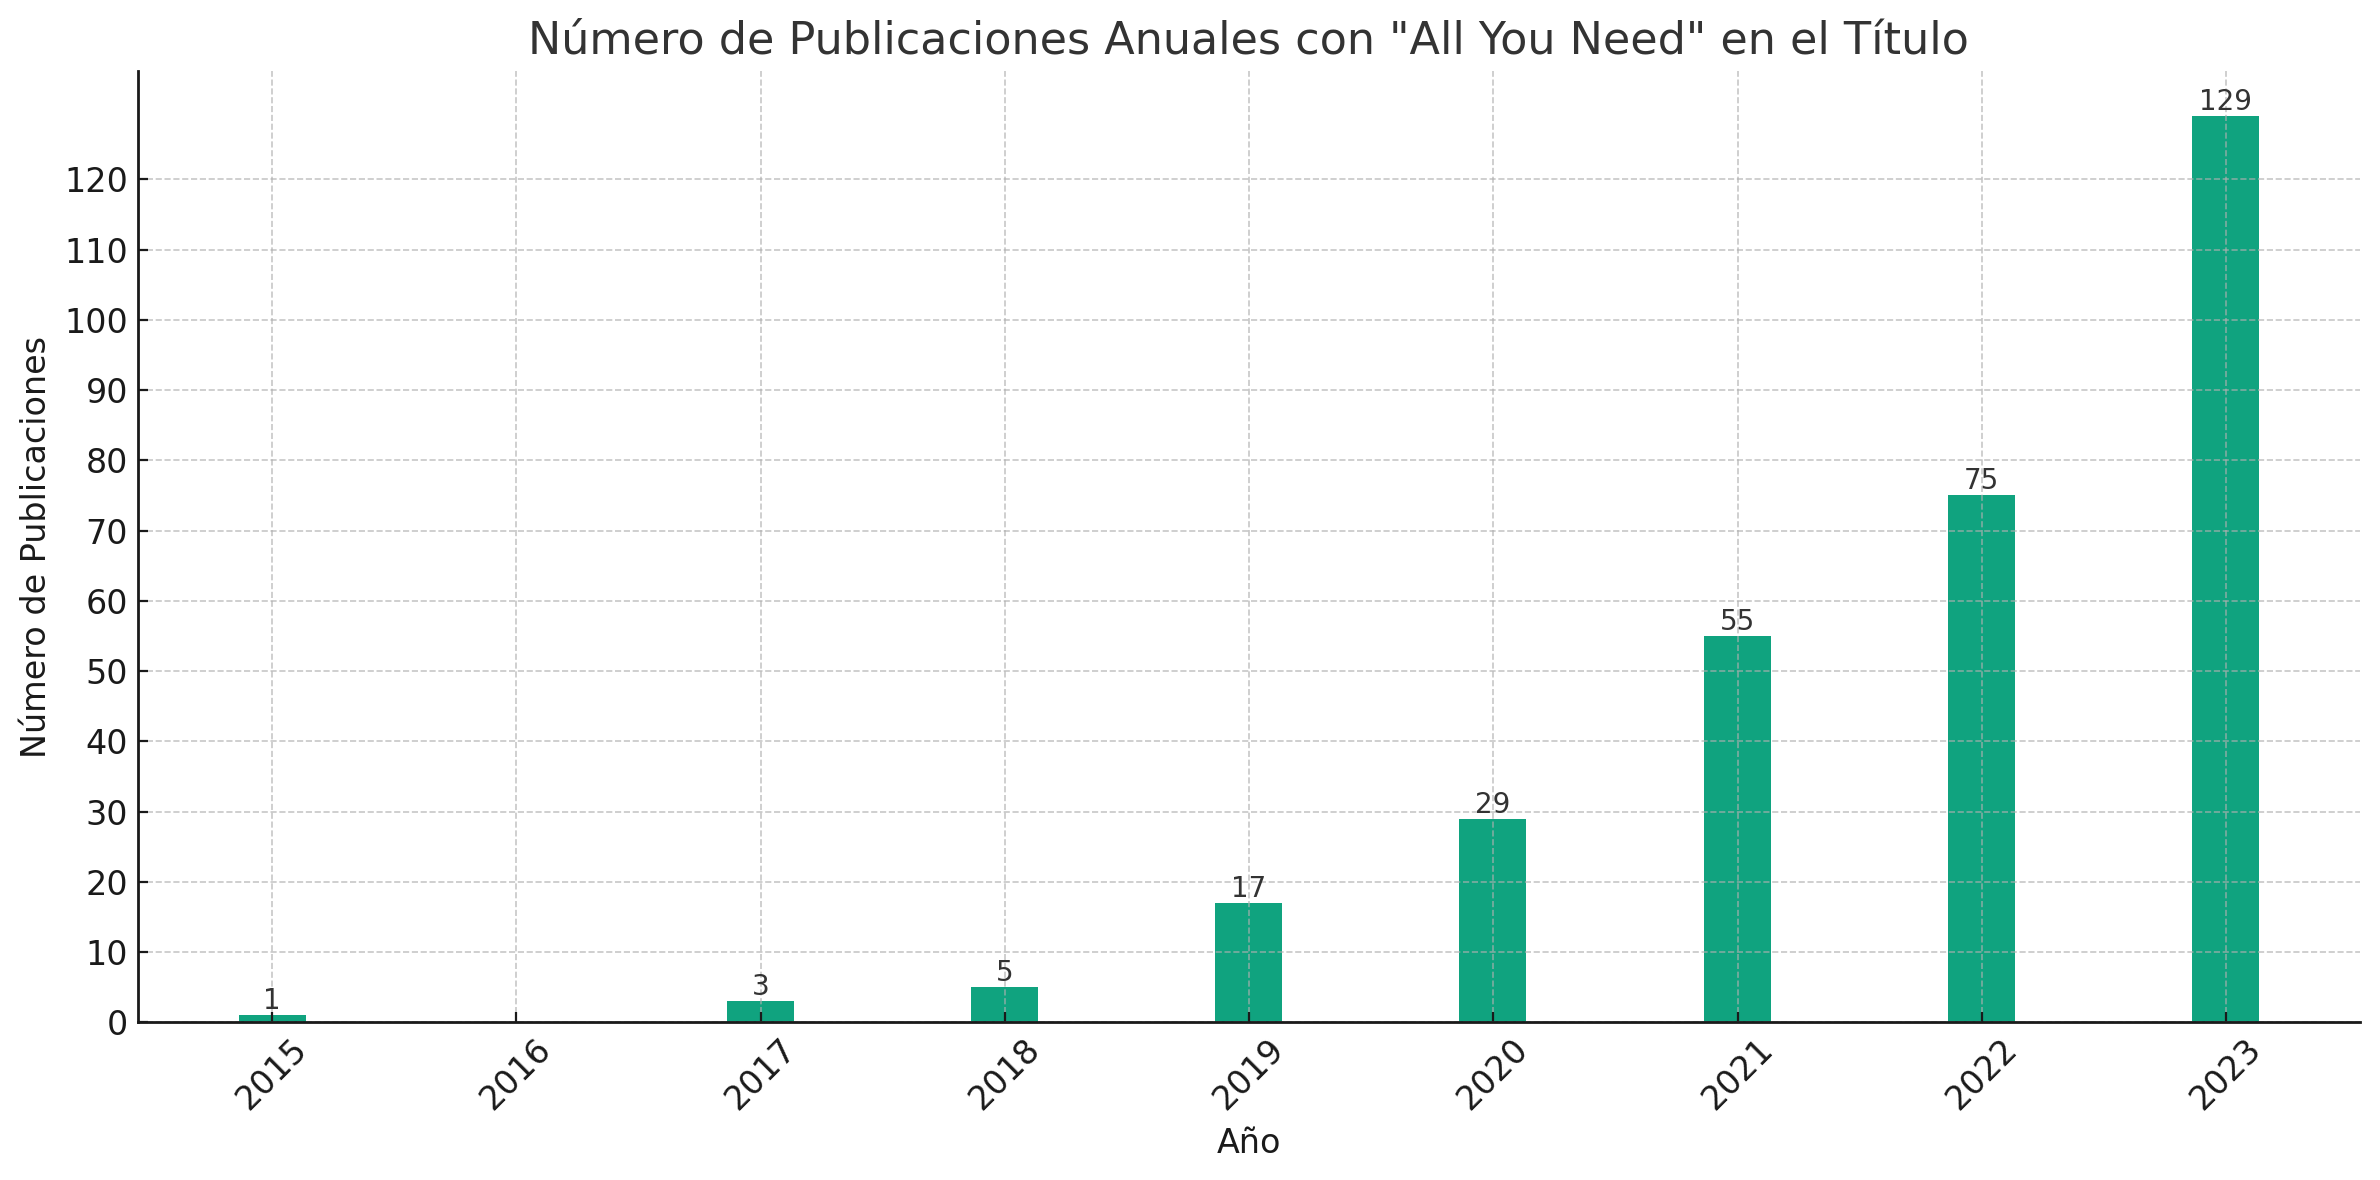
\includegraphics[width=0.9\textwidth]{./figuras/all_you_need_publicacionies_anuales.png}
    \source{Elaboración propia a partir del listado de \url{https://github.com/KentoNishi/awesome-all-you-need-papers}}
    \label{fig:all_you_need_publicaciones}
\end{figure}




